% !TeX root = mos-he.tex

%%%%%%%%%%%%%%%%%%%%%%%%%%%%%%%%%%%%%%%%%%%%%%%%%%%%%%%%%%%%%%%%

\refstepcounter{problem}  % 41. The locomotive problem

%%%%%%%%%%%%%%%%%%%%%%%%%%%%%%%%%%%%%%%%%%%%%%%%%%%%%%%%%%%%%%%%

\begin{prob}{הקצה הקצר של המקל}{S}{(The little end of the stick)}

אתה שובר מספר גדול של מקלות זכוכית באורך $1$ לשני חלקים. למקום השבירה התפלגות אחידה לאורך המקל.


\que{1} 
מה התוחלת של אורכו של החלק 
\textbf{הקטן}
יותר?

\que{2} 
מה התוחלת של היחס בין אורכו של החלק הקטן לאורכו של החלק הגדול?
\end{prob}
\solution{}

\ans{1}
ההסתברות שנקודת השבירה היא בצד השמאלי של המקל היא
$1/2$
שהיא גם ההסתברות שהנקודה בצד ימין. החלק הקטן יותר נמצא באותו צד שבו נמצאת נקודת השבירה. התוחלת של נדוקת השבירה היא באמצע בין קצה המקל לבין אמצע המקל:
\[
E(\textrm{יותר הקטן אורך}) = \frac{1}{2}\cdot\frac{1}{2}=\frac{1}{4}\,.
\]

\ans{2}
ללא הגבלת הכלליות הנח שנקודת השבירה נמצאת בצד הימני של המקל (איור%
~\ref{f.stick}).
היחס בין החלק הקטן והחלק הגדול הוא
$(1-x)/x$
ואורכו של החלק הגדול מתפלג אחיד בתוך
$(1/2,1)$. 
לכן:
\begin{eqn}
E(\textrm{יותר קטן / יותר גדול יחס})&=&\left(\frac{1}{1-(1/2)}\right)\int_{1/2}^1 \frac{1-x}{x} \,dx\\
&=& 2\int_{1/2}^1 \left(\frac{1}{x} -1\right) \,dx \\
&=& 2\left.(\ln |x| - x)\right|_{1/2}^1 = 2\ln 2 -1\approx 0.3863\,.
\end{eqn}
\begin{figure}[tb]
\begin{center}
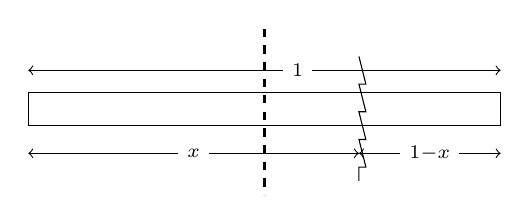
\begin{tikzpicture}
\draw (0,0) -- ++(6,0) -- ++(0,12pt) -- ++(-6,0) -- cycle;
\draw[<->] (0,20pt) --
  node[fill=white,xshift=12pt] {$\scriptstyle 1$} ++(6,0);
\draw[decorate,decoration=saw] (4.2,25pt) -- +(0,-45pt);
\draw[thick,dashed] (3,35pt) -- +(0,-60pt);
\draw[<->] (0,-10pt) --
  node[fill=white] {$\scriptstyle x$} (4.2,-10pt);
\draw[<->] (4.2,-10pt) --
  node[fill=white] {$\scriptstyle 1-x$} (6,-10pt);
\end{tikzpicture}
\end{center}
\caption{שבירת מקל לשני חלקים}\label{f.stick}
\end{figure}

\textbf{סימולציה}
\selectlanguage{english}
\begin{verbatim}
Expectation of length of smaller = 0.2500
Average length of smaller        = 0.2490
Expectation of smaller/larger    = 0.3863
Average smaller/larger           = 0.3845
\end{verbatim}
\selectlanguage{hebrew}

%%%%%%%%%%%%%%%%%%%%%%%%%%%%%%%%%%%%%%%%%%%%%%%%%%%%%%%%%%%%%%%%


\begin{prob}{המקל השבור}{D,S}{(The broken bar)}

אתה שובר מספר רב של מקלות זכוכית באורך 
$1$
בשתי נדוקות שבירה (איור%
~\ref{f.break1}).

\que{1} 
מה התוחלת של אורכו של החלק הקצר ביותר?

\que{2} 
מה התוחלת של אורכו של החלק הארוך ביותר?

\textbf{רמז:}
$x,y$
הם משתנים אקראים בלתי-תלויים בהתפלגות אחידה בתוך 
$(0,1)$.
ניתן להציג כל זוג
$(x,y)$
כנקודה בריבוע
$(0,1)\times (0,1)$ 
(איור%
~\ref{f.break2}).
מה ההסתברות ש-%
$(x,y) < (.5,.25)$? 

\textbf{Hint:}
עבור 
\que{1}
הנח שהחלק השמאלי הוא הקצר ביותר ועבור 
\que{2}
הנח שהחלק השמאלי הוא בארוך ביותר.
\begin{figure}[tb]
\centering
\selectlanguage{hebrew}
\subcaptionbox{%
חלוקת מקל לשני חלקים%
\label{f.break1}}
[.45\textwidth]
{
\centering
\begin{tikzpicture}[scale=.75]
\draw (0,0) node[below left] {$0$} --
  ++(6,0) node[below right] {$1$} --
  ++(0,12pt) -- ++(-6,0) -- cycle;
\draw[<->] (0,20pt) --
  node[fill=white] {$\scriptstyle 1$} ++(6,0);
\draw[decorate,decoration=saw] (1.8,25pt) -- +(0,-45pt);
\draw[decorate,decoration=saw] (4.7,25pt) -- +(0,-45pt);
\node[below left] at (1.8,0) {$x$};
\node[below left] at (4.7,0) {$y$};
\path (0,-3.5) rectangle +(0,3.5);
\end{tikzpicture}
}
\hspace{3em}
\subcaptionbox{%
יצוג האורכים במעגל היחידה%
\label{f.break2}}
[.45\textwidth]
{
\centering
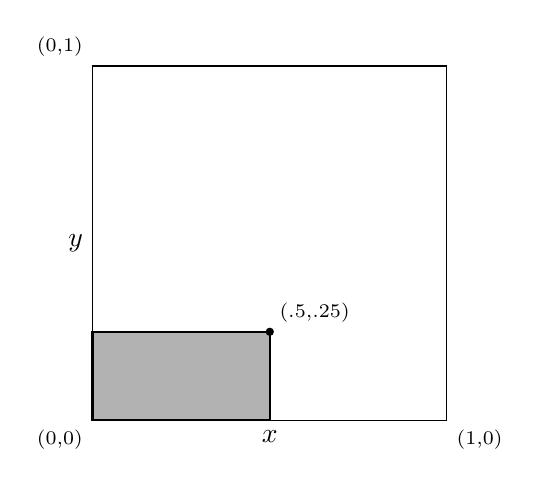
\begin{tikzpicture}[scale=.75]
\draw (-3,-3) rectangle +(6,6);
\draw[thick,fill=white!70!black] (-3,-3) -- ++(0,1.5) -- 
  ++(3,0) -- ++(0,-1.5) -- cycle;
\path (-3,-3) node[below left] {$\scriptstyle (0,0)$} --
  node[below] {$x$} (3,-3)
  node[below right] {$\scriptstyle (1,0)$};
\path (-3,-3) -- node[left] {$y$} (-3,3)
  node[above left] {$\scriptstyle (0,1)$};
\fill (0,-1.5) circle [radius=2pt]
  node[above right] {$\scriptstyle (.5,.25)$};
\end{tikzpicture}
}
\end{figure}
\end{prob}
\solution{}

\ans{1}
ללא הגבלת הכלליות הנח שהחלק השמאלי שאורכו 
$x$
הוא החלק הקצר ביותר. מכאן ש-%
$x<y-x$
ו-%
$x < 1-y$
שניתן לפשט ולקבל
$2x<y$
ו-%
$x+y<1$.

איור%
~\ref{f.shaded1}
מראה את הקווים
$y=2x$
(אדום) ו-%
$y=1-x$
(כחול). כדי לאמת את אי-השוויונות, 
$(x,y)$
חייבת להיות באיזור באפור לשמאל לשני הקווים. ניתן לחשב את נקודת החיתוך
$(1/2,2/3)$
על ידי פתרון שתי המשוואות.

הערכים של 
$(x,y)$
נמצאים בריבוע
$(0,1)\times(0,1)$,
ולכן יש לחשב את התוחלת מעל לתת-קבוצה האפורה של הריבוע על ידי חילוק האינטגרל בשטח של האיזור האפור
$\frac{1}{2} (\frac{1}{3}\cdot 1)=\frac{1}{6}$:
\begin{eqn}
E(x)&=& \frac{1}{1/6}\int_{0}^{1/3} x [(1-x)-2x]\,dx\\
&=&\int_{0}^{1/3} (6x -18x^2)\,dx\\
&=&\left. (3x^2-6x^3)\right|_0^{1/3}=\disfrac{2}{18}\approx 0.1111\,.
\end{eqn}

\begin{figure}[tb]
\centering
\selectlanguage{hebrew}
\subcaptionbox{%
איזור אפור עבור המקל הקצר ביותר%
\label{f.shaded1}}
[.45\textwidth]
{
\centering
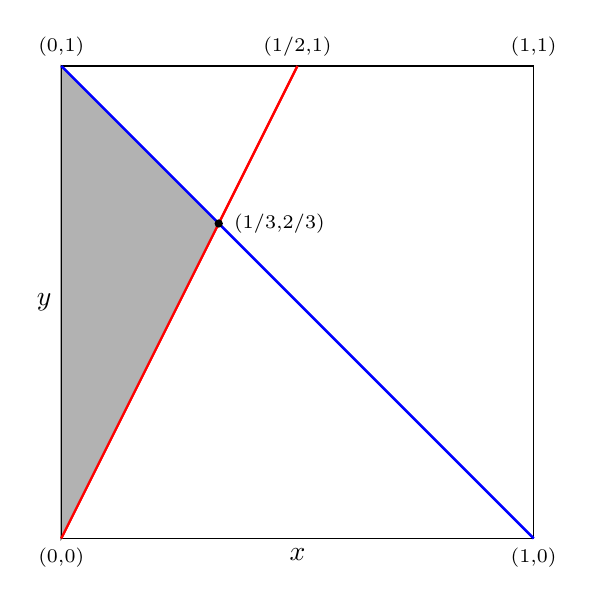
\begin{tikzpicture}[scale=1]
\draw (-3,-3) rectangle +(6,6);
\path (-3,-3) node[below] {$\scriptstyle (0,0)$} --
  node[below] {$x$} (3,-3)
  node[below] {$\scriptstyle (1,0)$};
\path (-3,-3) -- node[left] {$y$} (-3,3)
  node[above] {$\scriptstyle (0,1)$};
\draw[red,thick]  (-3,-3) -- (0,3);
\draw[blue,thick] (-3,3)  -- (3,-3);
\coordinate (P) at (-1,1);
\draw[fill=white!70!black] (-3,-3) -- (P) -- 
  (-3,3) -- cycle;
\draw[red,thick]  (-3,-3) -- (0,3);
\draw[blue,thick] (-3,3)  -- (3,-3);
\fill (P) circle[radius=1.5pt]
  node[right,xshift=2pt] {$\scriptstyle (1/3,2/3)$};
%\draw[thick,dotted] (-3,-3) -- (3,3);
\node[above] at(0,3) {$\scriptstyle (1/2,1)$};
\node[above] at(3,3) {$\scriptstyle (1,1)$};
\end{tikzpicture}
}
\hspace{1em}
\subcaptionbox{%
איזור אפור עבור המקל הארוך ביותר%
\label{f.shaded2}}
[.45\textwidth]
{
\centering
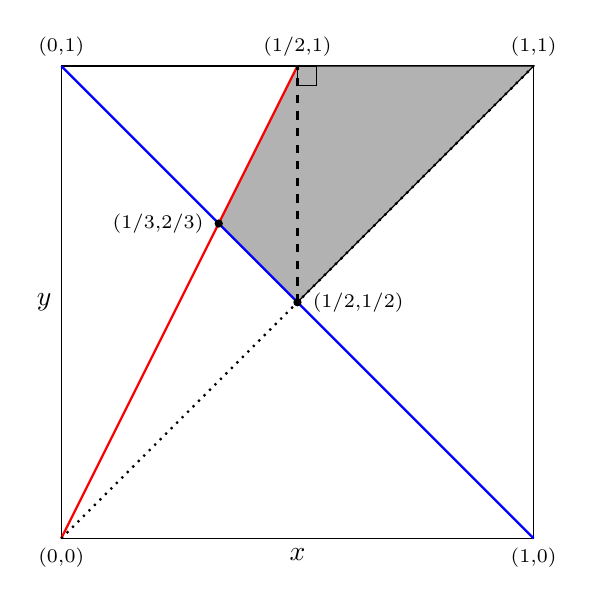
\begin{tikzpicture}[scale=1]
\draw (-3,-3) rectangle +(6,6);
\path (-3,-3) node[below] {$\scriptstyle (0,0)$} --
  node[below] {$x$} (3,-3)
  node[below] {$\scriptstyle (1,0)$};
\path (-3,-3) -- node[left] {$y$} (-3,3)
  node[above] {$\scriptstyle (0,1)$};
\coordinate (P) at (-1,1);
\coordinate (Q) at (0,0);
\draw[fill=white!70!black] (3,3) -- (Q) -- 
  (P) -- (0,3) -- cycle;
\draw[red,thick]  (-3,-3) -- (0,3);
\draw[blue,thick] (-3,3)  -- (3,-3);
\fill (P) circle[radius=1.5pt]
  node[left,xshift=-2pt] {$\scriptstyle (1/3,2/3)$};
\draw[thick,dotted] (-3,-3) -- (3,3);
\fill (Q) circle[radius=1.5pt]
  node[right,xshift=2pt] {$\scriptstyle (1/2,1/2)$};
\node[above] at(0,3) {$\scriptstyle (1/2,1)$};
\node[above] at(3,3) {$\scriptstyle (1,1)$};
\draw[thick,dashed] (Q) -- ++(0,3);
\draw (0,3cm-7pt) rectangle +(7pt,7pt);
\end{tikzpicture}
}
\end{figure}

\ans{2}
כדי שהחלק השמאלי יהיה הארוך ביותר 
$x>y-x$
ו-%
$x>1-y$, 
ולכן
$(x,y)$
חייבת להיות לימינו של
$y=2x$
(אדום) ולימינו של
$y=1-x$
(כחול) (איור%
~\ref{f.shaded2}).
בנוסף, לפי הנחה ש-%
$x$
נמצא לשמאלו של
$y$,
$(x,y)$
חייבת להיות לשמאלו של
$y=x$
(מנוקד).

כדי להקל על החישוב נחלק את האיזור האפור לשני משולשים (מקווקו) ונחשב את התוחלת בנפרד בשניהם. השטח של האיזור האפור מתקבל כסכום השטחים של המשולשים
$1/24+1/8=1/6$.
מכאן:
\begin{eqn}
E(\textrm{השמאלי במשולש}\;x)&=& 6\int_{1/3}^{1/2} x [2x-(1-x)]\,dx  \\
&=&\int_{1/3}^{1/2} \left(18x^2-6x\right)\,dx\\
&=&\left. (6x^3-3x^2)\right|_{1/3}^{1/2}=\disfrac{1}{9}\\
E(\textrm{הימני במשולש}\;x)&=& 6\int_{1/2}^{1} x [1-x]\,dx\\
&=&\int_{1/2}^{1} (6x-6x^2)\,dx\\
&=&\left. \left(3x^2-2x^3\right)\right|_{1/2}^{1}= \disfrac{1}{2}\\
E(x)&=& \disfrac{1}{9}+\disfrac{1}{2} = \disfrac{11}{18}\approx 0.6111\,.
\end{eqn}

התוחלת של אורכו של החלק הבינוני היא
$1-\frac{2}{18}-\frac{11}{18}=\frac{5}{18}\approx 0.2778$.

\textbf{סימולציה}
\selectlanguage{english}
\begin{verbatim}
Expectations: shortest = 0.1111, middle = 0.2778, longest = 0.6111
Averages:     shortest = 0.1115, middle = 0.2783, longest = 0.6102
\end{verbatim}
\selectlanguage{hebrew}

%%%%%%%%%%%%%%%%%%%%%%%%%%%%%%%%%%%%%%%%%%%%%%%%%%%%%%%%%%%%%%%%

\begin{prob}{לנצח במשחק לא-הוגן}{D,S}{(Winning an unfair game)}

נתון מטבע לא-הוגנת שההסתברות לעץ היא 
$1/3 < p < 1/2$. 
הטל את המטבע מספר זוגי של פעמים
$N=2n$.
אתה מנצח אם ורק אם 
\textbf{ביותר}
ממחצית ההטלטת מופיע עץ.

\que{1}
פתח נוסחה עבור ההסתברות לנצח 
$P_N$
ונוסחה עבור ההסתברות לתיקו
$T_N$.

\que{2}
פתח נוסחה עבור ה-%
$N$
עבורו יש את ההסתברות הגבוהה ביותר לנצח.

\textbf{רמז:} 
אם ההסתברות הגבוהה ביותר לנצח היא ב-%
$N$
הטלות אזי 
$P_{N-2} \leq P_N$
ו-%
$P_N\geq P_{N+2}$.
\end{prob}
\solution{}

\ans{1} 
כדי לנצח, עץ חייב להופיע ב-%
$i\in\{n+1, n+2, \ldots, 2n-1, 2n=N\}$
הטלות. מההתפלגות הבינומית:
\begin{eqn}
P_N &=& \sum_{i=n+1}^{2n} \dischoose{2n}{i} p^i (1-p)^{2n-i}\\
T_N &=& \dischoose{2n}{n} p^n (1-p)^{n}\,.
\end{eqn}

\ans{2}
כדי שההסתברות הגבוהה ביותר תהיהעבור
$N=2n$
חייב להתקיים:
\[
P_{2n-2} \leq P_{2n} \quad \textrm{ו-} \quad P_{2n}\geq P_{2n+2}\,.
\]
מתי
$P_{2n-2}\not = P_{2n}$?

\textbf{מקרה 1:}
לאחר הטלה
$2n-2$,
עץ הופיע 
$n$
פעמים ופלי
$n-2$
פעמים (כך שהיית זוכה אם היית עוצר כאן), אבל פלי מופיע בשתי ההטלות הבאות. עכשיו יש
$n$
עץ ו-%
$n$
פלי ולכן אתה מפסיד. ההסתברות היא:
\[
\dischoose{2n-2}{n}p^n(1-p)^{n-2} (1-p)^2\,.
\]

\textbf{מקרה $2$:}
לאחר הטלה
$2n-2$,
עץ הופיע 
$n-1$
פעמים ופלי
$n-1$
פעמים (כך שהיית מפסיד אם היית עוצר כאן), אבל עץ מופיע בשתי ההטלות הבאות. עכשיו יש
$n+1$
עץ ו-%
$n-1$
פלי ולכן אתה מנצח. ההסתברות היא:
\[
\dischoose{2n-2}{n-1}p^{n-1}(1-p)^{n-1} p^2\,.
\]
כדי לאמת את
$P_{2n-2}\leq P_{2n}$,
$P_{2n-2}$
לא יכול לגדול כאשר 
$P_{2n}$
נשאר ללא שינוי (מקרה $1$), אבל 
$P_{2n}$
יכול לגבול עד שהיא גבוהה מ-%
$P_{2n-2}$ (מקרה 2).
לכן:
\begin{eqn}
\dischoose{2n-2}{n}p^n(1-p)^{n-2} (1-p)^2 &\leq&
\dischoose{2n-2}{n-1}p^{n-1}(1-p)^{n-1} p^2\\
\disfrac{1}{n} (1-p) &\leq& \disfrac{1}{n-1} p\\
(n-1)(1-p) &\leq& np\\
n &\leq& \disfrac{1-p}{1-2p}\\
2n &\leq& \disfrac{1}{1-2p}+1\,.
\end{eqn}
באופן דומה, כדי לאמת את
$P_{2n}\geq P_{2n+2}$
חייב להיול ש:
\begin{eqn}
\dischoose{2n}{n+1}p^{n+1}(1-p)^{n-1}  (1-p)^2 &\geq&
\dischoose{2n}{n}p^{n}(1-p)^{n}  p^2\\
\disfrac{1}{n+1} (1-p) &\geq& \disfrac{1}{n} p\\
n(1-p)&\geq& (n+1)p\\
n &\geq& \disfrac{p}{1-2p}\\
2n &\geq&\disfrac{1}{1-2p}-1\,.
\end{eqn}
לכן, ערך עבור
$N=2n$
שעבורו מתקבל ההסתברות הגבוהה ביותר הוא המספר השלם הזוגי הקרוב ביותר ל-%
$1/(1-2p)$.
הקורא מוזמן להראות שאם
$1/(1-2p)$
אי-זוגי אזי
$P_{2n}=P_{2n+2}$.

\textbf{סימולציה}
\selectlanguage{english}
\begin{verbatim}
For probability             = 0.3700
Optimal games to be played  = 4
For  2 games, average won   = 0.1372
For  4 games, average won   = 0.1445
For  6 games, average won   = 0.1431

For probability             = 0.4000
Optimal games to be played  = 6
For  4 games, average won   = 0.1820
For  6 games, average won   = 0.1845
For  8 games, average won   = 0.1680

For probability             = 0.4500
Optimal games to be played  = 10
For  8 games, average won   = 0.2671
For 10 games, average won   = 0.2646
For 12 games, average won   = 0.2640
\end{verbatim}
\selectlanguage{hebrew}

%%%%%%%%%%%%%%%%%%%%%%%%%%%%%%%%%%%%%%%%%%%%%%%%%%%%%%%%%%%%%%%%

\begin{prob}{ממוצע של מספר ההתאמות}{S}{(Average number of matches)}
סדר חפיסת קלפים בשורה בסדר הסטנדרטי ואז סדר חפיסה שניה שורה בסדר אקראי מתחת לשורה הראשונה (איור%
~\ref{f.cards}).
מה התוחלת של מספר ההתאמות של קלף בשורה הראשונה עם קלף בשורה מתחתיו?
\end{prob}
\begin{figure}[tb]
\begin{center}
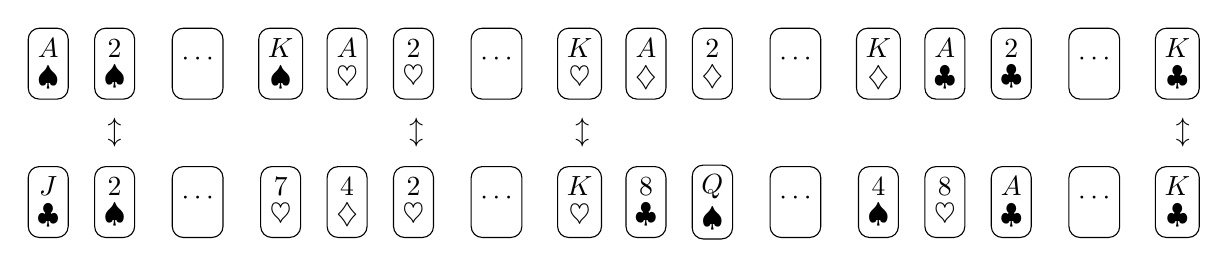
\begin{tikzpicture}
\foreach \x/\v/\s in {
  0/A/\spadesuit,
  1/2/\spadesuit,
  2.25/\cdots/,
  3.5/K/\spadesuit,
  4.5/A/\heartsuit,
  5.5/2/\heartsuit,
  6.75/\cdots/,
  8/K/\heartsuit,
  9/A/\diamondsuit,
  10/2/\diamondsuit,
  11.25/\cdots/,
  12.5/K/\diamondsuit,
  13.5/A/\clubsuit,
  14.5/2/\clubsuit,
  15.75/\cdots/,
  17/K/\clubsuit}
  \node[minimum height=9mm,draw,rounded corners]
    at (\x*24pt,0) {\shortstack{$\v$\\$\s$}};

\foreach \x/\v/\s in {
  0/J/\clubsuit,
  1/2/\spadesuit,
  2.25/\cdots/,
  3.5/7/\heartsuit,
  4.5/4/\diamondsuit,
  5.5/2/\heartsuit,
  6.75/\cdots/,
  8/K/\heartsuit,
  9/8/\clubsuit,
  10/Q/\spadesuit,
  11.25/\cdots/,
  12.5/4/\spadesuit,
  13.5/8/\heartsuit,
  14.5/A/\clubsuit,
  15.75/\cdots/,
  17/K/\clubsuit}
  \node[minimum height=9mm,draw,rounded corners]
    at (\x*24pt,-50pt) {\shortstack{$\v$\\$\s$}};

\node at (24pt,-25pt) {$\updownarrow$};
\node at (133pt,-25pt) {$\updownarrow$};
\node at (193pt,-25pt) {$\updownarrow$};
\node at (410pt,-25pt) {$\updownarrow$};
\end{tikzpicture}
\end{center}
\caption{התאמת שתי חפיסות קלפים}\label{f.cards}
\end{figure}
\solution{}

ההתפלגות אחידה כי לכל קלף בשורה השניה אותה המסתברות להתאים לקלף מעליו. לכן:
\[
E(\textrm{ההתאמות מספר}) = 52\cdot \frac{1}{52} = 1\,.
\]
\selectlanguage{english}
\begin{verbatim}
Expectation of matches = 1.00
Average of matches     = 1.01
\end{verbatim}
\selectlanguage{hebrew}

%%%%%%%%%%%%%%%%%%%%%%%%%%%%%%%%%%%%%%%%%%%%%%%%%%%%%%%%%%%%%%%%

\begin{prob}{הסתברויות של התאמות}{S}{(Probabilities of matches)}

סדר חפיסת קלפים בשורה בסדר הסטנדרטי ואז סדר חפיסה שניה שורה בסדר אקראי מתחת לשורה הראשונה (איור%
~\ref{f.cards}).
פתח נוסחה עבור 
$P(n,r)$,
ההסתברות שיהיו בדיוק 
$r$
התאמות של קלף בשורה הראשונה עם קלף בשורה מתחתיו? הנח ש-%
$P(k,0)$
נתון עבור
$0\leq k\leq n$.
\end{prob}
\solution{}

במבט ראשון נראה שבעיה זו דומה לבעיה~28 אבל קיים הבדל מהותי. השליפות המקופסאות הן בלתי-תלויות אבל כאן ההתאמות תלויות אחת בשניה. למשל, אם יש התאמה בקלף הראשון (בהסתברות 
$1/n$),
ההסתברות של התאמה בקלף השני היא
$1/(n-1)$.

ההסתברות שקבוצה 
\textbf{נתונה}
של
$r$
קלפים מתאימות היא:
\begin{equation}\label{eq.r-match}
\disfrac{1}{n}\cdot \disfrac{1}{n-1}\cdot \cdots \cdot \disfrac{1}{n+r-1}\,.
\end{equation}
כדי לקבל בדיוק 
$r$
התאמות, יש להכפיל משוואה%
~\ref{eq.r-match}
ב-%
$P(n-r,0)$,
ההסתברות שאין בכלל התאמות בשאר 
$n-r$
הקלפים. לבסוף, יש 
${n\choose r}$
דרכים לבחור
$r$
התאמות, ולכן:
\begin{eqn}
P(n,r)&=& \dischoose{n}{r}\disfrac{1}{n(n-1)(n+r-1)} P(n-r,0)\\
&=& \disfrac{n!}{r!(n-r)!}\cdot\disfrac{1}{n!/(n-r)!}P(n-r,0)\\
&=&\disfrac{1}{r!}P(n-r,0)\,.
\end{eqn}
נוסחה זו פותרת את הבעיה כי 
$P(k,0)$
נתונה.

\L{Mosteller}
מפתח נוסחה סגורה וגבול עבור
$P(n,r)$:
{
\addtolength{\arraycolsep}{-3pt}
\begin{eqnarray}
P(n,k)&=&\disfrac{1}{k!}\sum_{i=0}^{n-k} \disfrac{(-1)^i}{i!}\\
\label{eq.r-matches-lim}
\lim_{n-r\rightarrow \infty} P(n,k)&\approx& \disfrac{1}{k!}e^{-1}\,.
\end{eqnarray}
}

\textbf{סימולציה}

הרצתי את הסימולציה עבור 
$n=52$
קלפים וחישבתי את ההסתברות ממשוואה%
~\ref{eq.r-matches-lim}.
\selectlanguage{english}
\begin{verbatim}
Probability of 1 matches = 0.3679
Proportion 1 matches     = 0.3710
Probability of 2 matches = 0.1839
Proportion 2 matches     = 0.1828
Probability of 3 matches = 0.0613
Proportion 3 matches     = 0.0569
Probability of 4 matches = 0.0153
Proportion 4 matches     = 0.0168
\end{verbatim}
\selectlanguage{hebrew}

%%%%%%%%%%%%%%%%%%%%%%%%%%%%%%%%%%%%%%%%%%%%%%%%%%%%%%%%%%%%%%%%

\begin{prob}{לבחור את הנדוניה הגדול ביותר}{D,S}{(Choosing the largest dowry)}

הנח סידרה של 
$n$
קלפים עם הפנים למטה. על פניו של כל קלף נמצא מספר שלם חיובי אבל אין מידע על ההתלפגות שלהם. הפוך את הקלפים אחד-אחד ועיין במספרים. לאחר חשיפת כל אחד מהקלפים, אתה יכול להכריז שמספר זה הוא הגדול ביותר בסידרה. אם אתה צודק אתה מנצח, אחרת אתה מפסיד. למשל, אם הסדרה היא 
$(47, 23, 55, 4)$,
אתה מנצח רק אם אתה בוחר שת הקלף השלישי.

הנה אסטרטגיה: ל-%
$r$
קבוע, וותר על
$r-1$
הקלפים הראשונים ובחר את הקלף הראשון שמספרו גדול מכל 
$r-1$
הקלפים.

\que{1}
עבור
$n=4$
ו-%
$r=3$
בדוק את כל התמורות ומצא בכמה מהם את מנצח.

\que{2}
פתח נוסחה עבור ההסתברות לניצחון עבור 
$n, r$
שרירותיים.

\que{3} מצא קירוב להסתברות כאשר 
$n,r\rightarrow \infty$.

\textbf{רמז:}
נתון
$r$
באיזה מקומות יכול להופיע המספר הגדול ביותר
$m$
ובאיזה מקומות המספרים שהם פחות או שווים ל-%
$m$? 

\end{prob}
\solution{}

\ans{1}
כדי לפשט את הסימון נכתוב את דירוג מספרים כ-%
$1,2,3,4$
למרות שהערכים אמיתיים של המספרים לא ידועים, ולמשל יכולים להיות 
$4,23,47,55$.
אם אתה חושף קלפים
$1,2,3$
(שהם בעצם
$4,23,47$),
אינך יודע אם לבחור
$47$
או לחכות ובחור את הקלף האחרון.

יש 
$24$
תמורות של ארבעה מספרים. לפי האסטרטגיה אתה מוותר על שני הקלפים הראשונים ובוחר או את הקלף השלישי או את הקלף הרביעי, כך שאתה מפסיד אם $4$ נמצא במקום הראשון של התמורה. מה עם התמורה
$(1,2,3,4)$?
אתה מוותר על
$1,2$
ובוחר 
$3$
בגלל שהוא גובהה יותר מ-%
$1,2$
אבל אתה מפסיד כי זה לא המספר הגדולה ביותר. מה עם התמורה
$(1,3,2,4)$?
שוב, לפי האסטרטגיה אתה מוותר על
$1,3$,
אבל מוותר גם על
$2$
כי הוא 
\textbf{לא}
גדול יותר מ-%
$1,3$.
כעת אתה בוחר
$4$
ומנצח. נסח טיעונים דומים לכל התמורות ובדוק שכל התמורות עם 
$4$
במסגרת הן נצחונות:
\[
\addtolength{\arraycolsep}{-2pt}
\renewcommand*{\arraystretch}{1.5}
\begin{array}{cc|cc@{\hspace{2em}}cc|cc@{\hspace{2em}}cc|cc@{\hspace{2em}}cc|cc@{\hspace{2em}}cc|cc@{\hspace{2em}}cc|cc}
1&2\;&\;3&4&
1&2\;&\;\fbox{$4$}&3&
1&3\;&\;2&\fbox{$4$}&
1&3\;&\;\fbox{$4$}&2&
1&4\;&\;2&3&
1&4\;&\;3&2\\
2&1\;&\;3&4&
2&1\;&\;\fbox{$4$}&3&
2&3\;&\;1&\fbox{$4$}&
2&3\;&\;\fbox{$4$}&1&
2&4\;&\;1&3&
2&4\;&\;3&1\\
3&1\;&\;2&\fbox{$4$}&
3&1\;&\;\fbox{$4$}&2&
3&2\;&\;1&\fbox{$4$}&
3&2\;&\;\fbox{$4$}&1&
3&4\;&\;2&1&
3&4\;&\;2&1\\
4&1\;&\;2&3&
4&1\;&\;3&2&
4&2\;&\;1&3&
4&2\;&\;3&1&
4&3\;&\;1&2&
4&3\;&\;2&1
\end{array}
\]
ההסתברות לנצח היא
$10/24$.

\ans{2}
אתה מפסיד אם המספר הגדול ביותר נמצא באחד המקומות
$1,\ldots,r-1$.
לכן כדי לנצח מספר הגדול ביותר חייב להיות במקום
$m$
כאשר
$r\leq m\leq n$:
\[
1\quad 2\quad \cdots\quad r-2 \quad r-1 \quad \overbrace{r \quad r+1 \quad \cdots\quad m-1\quad  m \quad m+1\quad \cdots \quad n}^{\textrm{כאן להיות חייב ביותר גדול מספר}}\,.
\]
לפי האסטרטגיה אתה מוותר על
$r-1$
הקלפים הראשונים. אתה תבחר מקום
$m$
אם ורק אם 
\textbf{כל}
במספרים ב-%
$(r,\ldots,m-1)$
קטנים מ%
\textbf{כל}
המספרים ב-%
$(1,\ldots,r)$.
במילים אחרות, המספר הגדול ביותר בסידרה
$(1,\ldots,m-1)$
הוא
\textbf{לא}
בחלק השני של הסידרה
$(r,\ldots m-1)$
אלא בחלק הראשון
$(1,\ldots,r-1)$.
ההסתברות היא:
\[
P((1,\ldots,r-1)\textrm{ב- נמצא}\;(1,\ldots,m-1)\textrm{ב- ביותר הגדול המספר}) = \disfrac{r-1}{m-1}\,.
\]
ההסתברות שהמספר הגדול ביותר נמצא ב-%
$m$
הוא
$1/n$
ולכן:
\begin{equation}\label{eq.dowry1}
P(\textrm{ניצחון}) = \sum_{m=r}^{n} \disfrac{1}{n} \cdot \disfrac{r-1}{m-1}= \disfrac{r-1}{n}\sum_{m=r}^{n} \disfrac{1}{m-1}\,.
\end{equation}
עבור
$n=4, r=3$, $P(\textrm{ניצחון}) = 5/12=10/24$.

משוואה%
~\ref{eq.dowry1}
לא מוגדרת עבור
$r=1$
אבל ההסתברות לנצח כאשר אתה בוחר את המספר הראשון הוא
$1/n$.
לערך גבוהה ביותר של
$r$
יש הסתברות גבוהה יותר כפי שראינו בדוגמה.

\ans{3}
נכתוב משוואה%
~\ref{eq.dowry1}
כך:
\begin{equation}\label{eq.dowry2}
P(\textrm{ניצחון}) =\disfrac{r-1}{n}\left(\sum_{m=2}^{n} \disfrac{1}{m-1}-\sum_{m=2}^{r-1} \disfrac{1}{m-1}\right)\,.
\end{equation}
עבור 
$n,r$
גדולים, ניתן למצוא קירוב למשוואה%
~\ref{eq.dowry2}
כך:
\[
P(\textrm{ניצחון})=\disfrac{r}{n}(\ln n - \ln r)=\disfrac{r}{n}\ln \disfrac{n}{r}=-\disfrac{r}{n}\ln \disfrac{r}{n}\,.
\]
נסמן
$x=r/n$
ונמצא את המקסימום מהנגזרת:
\begin{eqn}
(-x\ln x)' &=& -x\cdot \frac{1}{x} + (-1) \ln x=0\\
\ln x &=& -1\\
x &=& 1/e\,.
\end{eqn}
כדי למקסם את ההסתברות לנצח בחר
$r \approx n/e$.

\textbf{סימולציה}

הרצתי את הסימולציה עם
$100$
קלפים וערכי
$r$
קרובים ל-%
$100/e$:
\selectlanguage{english}
\begin{verbatim}
Reject cards before r = 36:
Probability of wins   = 0.3674
Proportion wins       = 0.3641
Reject cards before r = 37:
Probability of wins   = 0.3678
Proportion wins       = 0.3759
Reject cards before r = 38:
Probability of wins   = 0.3679
Proportion wins       = 0.3548
Reject cards before r = 30:
Probability of wins   = 0.3590
Proportion wins       = 0.3601
\end{verbatim}
\selectlanguage{hebrew}

%%%%%%%%%%%%%%%%%%%%%%%%%%%%%%%%%%%%%%%%%%%%%%%%%%%%%%%%%%%%%%%%

\begin{prob}{בחירת המספר האקראי הגדול ביותר}{D,S}{(Choosing the largest random number)}

הנח סידרה של 
$n$
קלפים עם הפנים למטה. על פניו של כל קלף נמצא מספר ממשי עם התפלגות אחידה ב-%
$0.0\leq x<1.0$.
הפוך את הקלפים אחד-אחד ועיין במספרים. לאחר חשיפת כל אחד מהקלפים, אתה יכול להכריז שמספר זה הוא הגדול ביותר בסידרה. אם אתה צודק אתה מנצח, אחרת אתה מפסיד.

השתמש באסטרטגיה של בעיה~37: החלט על ערך
$r$
כך שאתה מוותר על 
$r-1$
הקלפים הראשונים ובוחר את הקלף הראשון שגדול מהמספר הגדול ביותר ב-%
$r-1$
קלפים הראשונים.

\textbf{הגדרה:}
$d$,
\textbf{ערך שווה-נפש},
הוא הערך שמתחתיו אתה מוותר על הקלף ומעליו את לבחור את הקלף.

\que{1} 
חשב את
$d$
עבור
$n=1$
וחשב את ההסתברות לנצח.

\que{2}
חשב את
$d$
עבור
$n=2$
וחשב את ההסתברות לנצח.

\que{3}
חשב את
$d$
עבור
$n=3$.
אל תנסה לחשב את ההסתברות לנצח!

\textbf{הערה:}
בבעיה~37 בערכים יכולים להיות
$100, 200, 300$ 
או
$100, 50, 20$
כך שחשיפת המספר הראשון לא מספק שום מידע על המספרים האחרים. בבעיה זו, ההתלפגות אחידה, ולכן אם המספר הראשון הוא 
$0.2$,
ההסתברות שהמספר השני יהיה גדול יותר היא 
$0.8$
ואם המספר הראשון הוא 
$0.8$
ההסתברות שהמספר השני יהיה גדול יותר היא
$0.2$.

\end{prob}
\solution{}

יהי
$v_1,v_2,v_3$
המספרים על שלושת הכרטיסים.

\ans{1}
אין ברירה אלא לבחור את הקלף הראשון כי אין קלפים אחרים. לכן אין ערך שווה-נפש. 
$v_1$
הוא המספר "הגדול ביותר",
$P({ניצחון})=1$.

\ans{2}
אם אתה בוחר את הקלף הראשון
$P(\textrm{ניצחון})=v_1$
שהיא ההסתברות שהמספר על הקלף השני קטן יותר. אם אתה מוותר על הקלף הראשון,
$P(\textrm{ניצחון})=1-v_1$
שהיא ההסתברות ש-%
$v_2>v_1$.
לכן, אם 
$v_1<0.5$ 
בחר את הקלף השני כי
$1-v_1>0.5$
ואם 
$v_1>0.5$
בחר את הקלף הראשון. מכאן ש-%
$d=0.5$.

הנה הנוסחה לחישוב ההסתברות לנצח:
\[
P(\textrm{ניצחון}) = p(\textrm{ניצחון} \,|\,v_1<0.5)\,p(v_1<0.5)+ p(\textrm{ניצחון}\,|\,v_1>0.5)\,p(v_1>0.5)\,.
\]
$p(v_1<0.5)=0.5$
נובע מההתפלגות האחידה. מה עם
$p(\textrm{ניצחון} \,|\,v_1<0.5)$? 
לפי האסטרטגיה אתה מנצח אם
$0.5<v_2<1$
אבל גם אם
$v_1<v_2<0.5$.
ההתפלגות של 
$v_1$
היא אחידה ב-%
$(0,0.5)$
ולכן:
\[
p(\textrm{ניצחון} \,|\,v_1<0.5)=\disfrac{1}{2} + \disfrac{1}{4}=\disfrac{3}{4}\,.
\]
ניתן לעשות חישוב דומה עבור
$v_1>0.5$.
נרכיב את כל החישובים הללו ביחד וקבל:
\[
P(\textrm{ניצחון})=\disfrac{3}{4}\cdot\disfrac{1}{2}+\disfrac{3}{4}\cdot\disfrac{1}{2}=\disfrac{3}{4}\,.
\]

\ans{3}
אם אתה בוחר את הקלף הראשון,
$P(\textrm{ניצחון})=v_1^2$
כי הקלף השני והשלישי חייבים להיות קטנים מהראשון.

אם אתה מוותר על הקלף הראשון ובוחר את השני כי 
$v_2>v_1$
אזי:
\begin{itemize}
\item $P(\textrm{ניצחון})=(1-v_1)v_1$
אם
$v_2>v_1$ 
ו-%
$v_3<v_1$.
\item $P(\textrm{ניצחון})=v_1(1-v_1)$
אם
$v_2<v_1$
ו-%
$v_3>v_1$.
\item $P(\textrm{ניצחון})=\frac{1}{2}(1-v_1)^2$
אם
$v_2>v_1$
ו-%
$v_3>v_1$,
כי ניצחון תלוי בסדר:
\\
אם הוא
$(0.55, 0.75, 0.65)$
אתה מנצח
ואם הוא
$(0.55, 0.65, 0.75)$
אתה מפסיד.
\end{itemize}

הערך שווה-נפש 
$d$
הוא ערך עבורו ההסתברות לנצח על ידי בחירת הקלף הראשון שווה להסתברות לנצח על ידי ויתור על הקלף הראשון:
\begin{eqn}
d^2 &=& 2d(1-d) + \frac{1}{2}(1-d)^2\\
5d^2 - 2d -1 &=&0\\
d&=& \disfrac{1+\sqrt{6}}{5}\approx 0.6899\,.
\end{eqn}
\L{Gilbert\&Mosteller \cite[page~55]{gilbert}}
מראים שעבור
$n=3$:
\[
P(\textrm{ניצחון}) = \disfrac{1}{3}+\disfrac{d}{2}+\disfrac{d^2}{1}-\disfrac{3d^3}{2}\approx 0.6617\,.
\]
\textbf{סימולציה}
\selectlanguage{english}
\begin{verbatim}
For  3 cards:
Indifference value = 0.6000
Probability of win = 0.6693
Proportion of wins = 0.6628
Indifference value = 0.6899
Probability of win = 0.6617
Proportion of wins = 0.6711
Indifference value = 0.7200
Probability of win = 0.6519
Proportion of wins = 0.6473
\end{verbatim}
\selectlanguage{hebrew}

%%%%%%%%%%%%%%%%%%%%%%%%%%%%%%%%%%%%%%%%%%%%%%%%%%%%%%%%%%%%%%%%
